\section{Graphics Card Simulations}

\par
Although the probabilistic approach described in the previous section is sufficient for S2 light, it has several significant limiting factors which make it unsuitable for other areas, including;
\begin{enumerate}
    \item requiring that optical simulations be performed at least once
    \item the maps created are only valid for that given detector set-up 
\end{enumerate}
As the photon propagation needs to be performed at least once, it does not scale well to other areas of the LZ detector; for example if a probabilistic map were to be used in the TPC Liquid Xenon, for similar statistics as the Gas Xenon, XXX photons would have to be simulated, which would equate to XXX CPU hours.
Although there are ways in which this could be reduced - such as Z-line symmetry - the initial overhead remains impractically high.
However, as the number of photons produced in an event are typically less for S1 than S2, it has not been as significant a bottleneck as S2 light.

\par
Instead we can consider more optimal approaches to performing the simulations, and whether invasions in other fields can lend a hand.
As optical photons are a fairly simple particle to simulation - daughter particles are not produced and interactions of material boundaries are the primary concern.
Simulations become dominated by intersection calculations; namely \textit{"has the photon reached the edge of this material yet?"}.

\par
The film and gaming industries have together given developed and improved ray-tracing capabilities which fundamentally are intersection calculations.


\begin{figure}[!htbp]
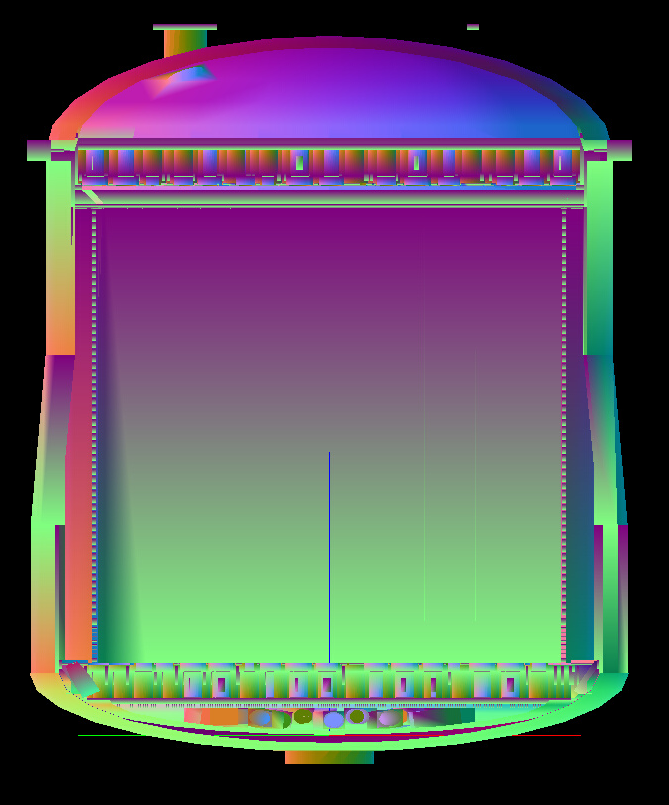
\includegraphics[width=8cm]{Figures/Simulations/LZ_In_Opticks.png}
\centering
\caption{TPC of LZ raytraced. Translated from Geant4 GDML file into NPY set using Opticks and viewed within Opticks via the OpenGL Buffer.
The blue, green and red lines towards the bottom of the figure are the axis.}
\label{fig:OpticksLZTPC}
\end{figure}

\par
To compare the optical photon propagation within the LZ geometry on Opticks with that from BACCARAT, a series of tests were devised.
As the initial purpose of this project was to simulate S2 photons, two S2 light maps were created using the same number of photons; XXXX million (15 billion I think).
Using a much of the same geometry as possible the simulations from BACCARAT and Opticks were compared.

\begin{figure}[!htbp]
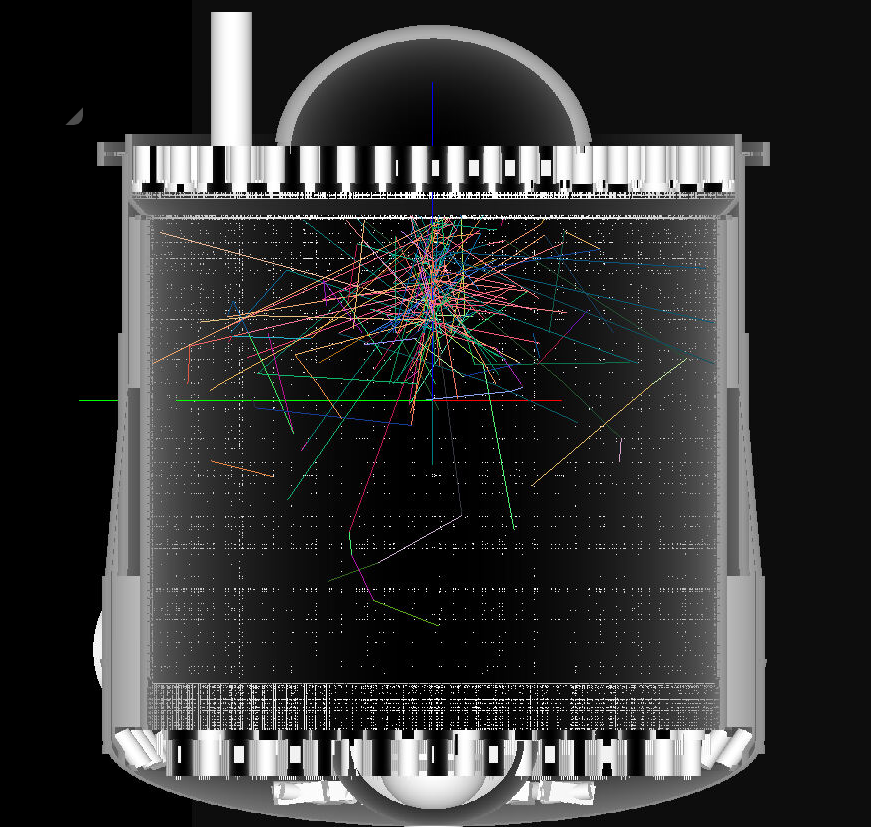
\includegraphics[width=10cm]{Figures/Simulations/LZ_S1_photons_In_Opticks.png}
\centering
\caption{TPC of LZ raytraced. Translated from Geant4 GDML file into NPY set using Opticks and viewed within Opticks via the OpenGL Buffer.
The blue, green and red lines towards the bottom of the figure are the axis.}
\label{fig:OpticksLZTPC_S1_Photons}
\end{figure}



\par
The LZ collaboration is continuing to develop upon this work with an integration plan into the simulation chain \cite{SEriksen_Opticks_CHEP_2021_ref}.
Additionally, as this work was performed using NVIDIA OptiX 6.5.0, newer features available in 7.0.0+ will allow even greater performance and better use of compute-cluster GPU setup.
TODO CITE.
The primary limitation has been upon an improved GDML writer and reader in Geant4, requireing the LZ simulation package to update. 
However, with the discussions of G3 direct detection dark matter experiments, the optical photons will continue to be a limitation and are already being considered \cite{DARWIN_GPU_simulations_2022}.




